\section{Mise en place}

\subsection*{Machine locale}

Cette partie de mise en place s'effectue sur la machine locale et non sur la machine cible / distante. Veuillez suivre pas-à-pas les différentes étapes. 

\subsubsection*{Installation de NodeJS}

\begin{enumerate}
    \item Installer NodeJS : \url{https://nodejs.org/en/download}
\end{enumerate}

\subsubsection*{Installation de Claude}

\begin{enumerate}
    \item Installer Claude : \url{https://claude.ai/download}
\end{enumerate}

\subsubsection*{Installation de GEPO}

\begin{enumerate}
    \item Cloner le depot Github depuis le lien suivant : \url{https://github.com/HerdiiiL/gepo.git}
    \item Lancer la commande suivante : \textbf{git clone https://github.com/HerdiiiL/gepo.git}
    \item Se rendre dans le dossier \textbf{gepo-mcp}
    \item Modifier le fichier \textbf{src/remote/index.js} 
    \item Remplacer l'adresse IP par celle de la machine distante
    \item Lancer la commande suivante : \textbf{npm install}
    \item Lancer la commande suivante : \textbf{npx tsc}
\end{enumerate}

\subsubsection*{Configuration de Claude}

\begin{enumerate}
    \item Ouvrir l'application "Claude"
    
    \item Se rendre dans les paramètres de l'application
    
    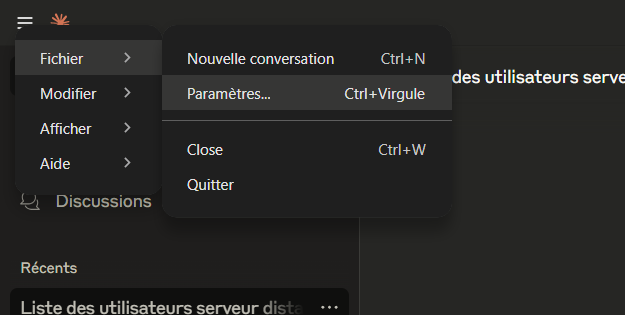
\includegraphics[width=0.6\textwidth]{../images/parametres-claude}
    
    \item Aller dans le section "Développeur"
    
    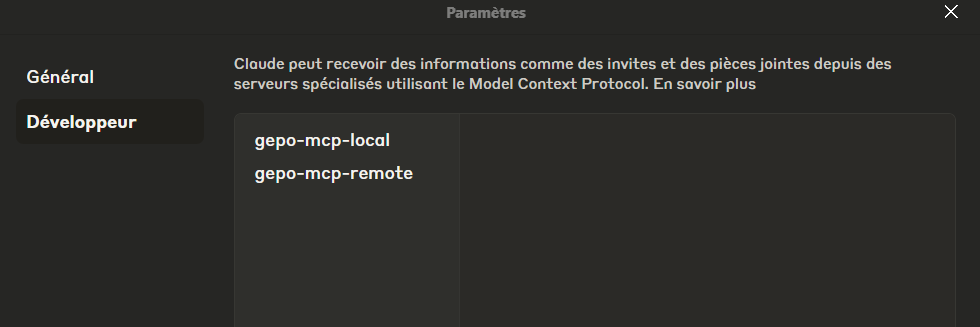
\includegraphics[width=0.6\textwidth]{../images/mode_developpeur-claude}
    
    \item Cliquer sur le bouton "Edit Config" ou "Modifier la configuration"
    
    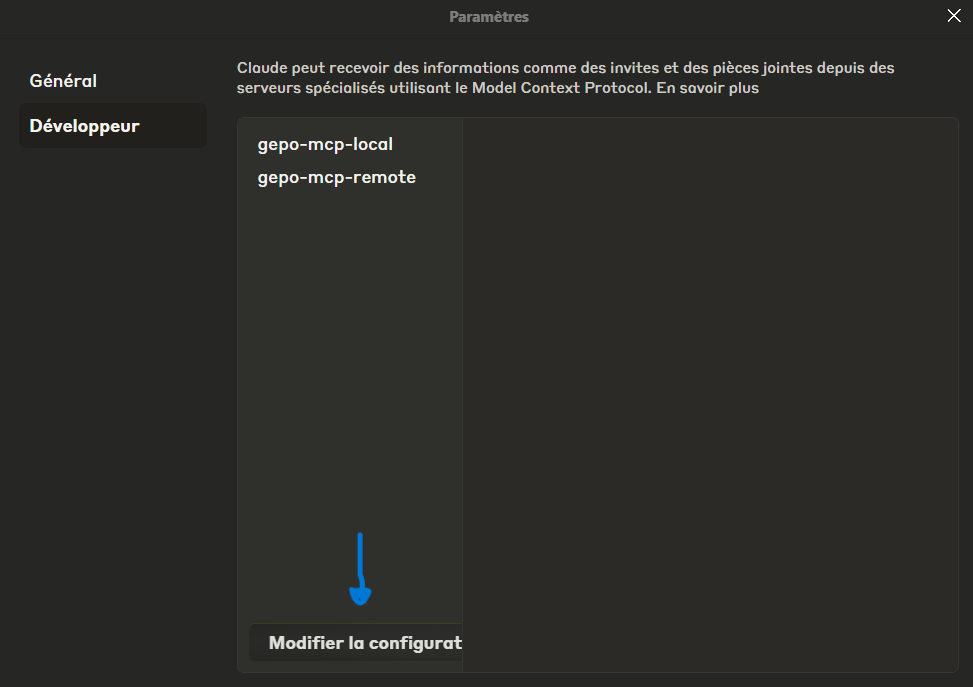
\includegraphics[width=0.6\textwidth]{../images/modifier_configuration-claude}

    \item En cliquant sur le bouton, un explorateur de fichiers devrait s'ouvrir
    
    \item Faire clique-droit sur le fichier \textbf{claude\_desktop\_config.json} et le modifier    
    \item Ajouter le contenu suivant : 
    
    \begin{lstlisting}[language=json,firstnumber=1]
    {
      "mcpServers": {
        "gepo-mcp-remote": {
          "command": "node", 
          "args": ["<emplacement_gepo>/gepo-mcp/build/remote/index.js"]
        }
      }
    }
    \end{lstlisting}

    \item Sauvegarder le fichier et quitter
    \item En redémarrant Claude, vous devriez voir la commande suivante apparaitre : \textbf{execute-ps-remote-command}
    
    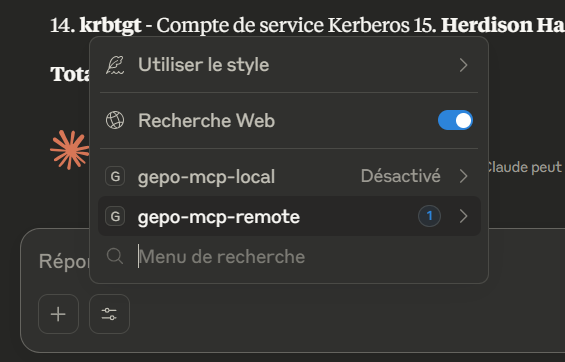
\includegraphics[width=0.6\textwidth]{../images/execute_ps_remote_command-claude}

    \item L'installation côté locale est terminée

\end{enumerate}

\subsection*{Serveur distant}

\begin{enumerate}
    \item Se rendre dans le dossier \textbf{gepo-mcp}
    \item Lancer la commande suivante : \textbf{npm install}
    \item Lancer la commande suivante : \textbf{node index.js}
    \item L'installation côté distant est terminée.
\end{enumerate}

\subsection*{Vérification}

\begin{enumerate}
    \item Ouvrir Claude et effectuer une commande en activant \textbf{execute-ps-remote-command}
\end{enumerate}